% Created 2019-05-17 vie 00:13
% Intended LaTeX compiler: pdflatex
\documentclass[11pt]{article}
\usepackage[utf8]{inputenc}
\usepackage[T1]{fontenc}
\usepackage{graphicx}
\usepackage{grffile}
\usepackage{longtable}
\usepackage{wrapfig}
\usepackage{rotating}
\usepackage[normalem]{ulem}
\usepackage{amsmath}
\usepackage{textcomp}
\usepackage{amssymb}
\usepackage{capt-of}
\usepackage{hyperref}
\author{Marco Centurion}
\date{\today}
\title{Usage Guide}
\hypersetup{
 pdfauthor={Marco Centurion},
 pdftitle={Usage Guide},
 pdfkeywords={},
 pdfsubject={},
 pdfcreator={Emacs 26.1 (Org mode 9.1.9)},
 pdflang={English}}
\begin{document}

\maketitle
\tableofcontents


\section{Description}
\label{sec:org17588f2}

This document is a brief manual of the software developed in the thesis "Model Driven Engineering applied to Network Configuration".

This guide will describe the basic steps to create a project that uses the  profile mdcms, create elements of a model using this profile, and finally execute the Model-to-Text transformation.

\section{Project}
\label{sec:org66c8ddb}

In order to create a Papyrus project that uses the model, the first step is to click on "File > New > Project":

\begin{center}
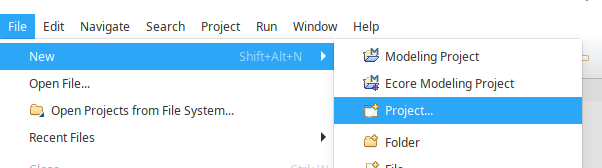
\includegraphics[width=.9\linewidth]{images/project_1.png}
\end{center}

Then you must choose the project type "Papyrus Project", within "Papyrus" category:

\begin{center}
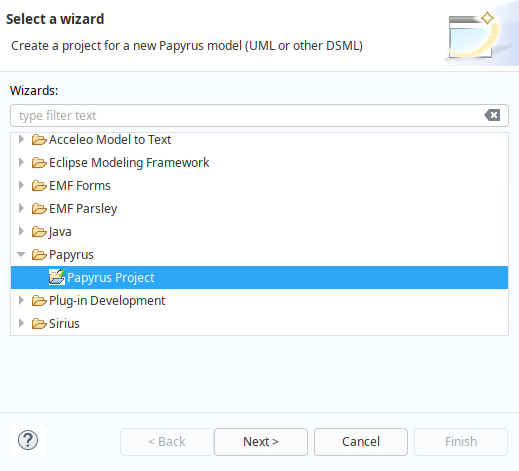
\includegraphics[width=.9\linewidth]{images/project_2.png}
\end{center}
\newpage

For the next step no changes need to be made:

\begin{center}
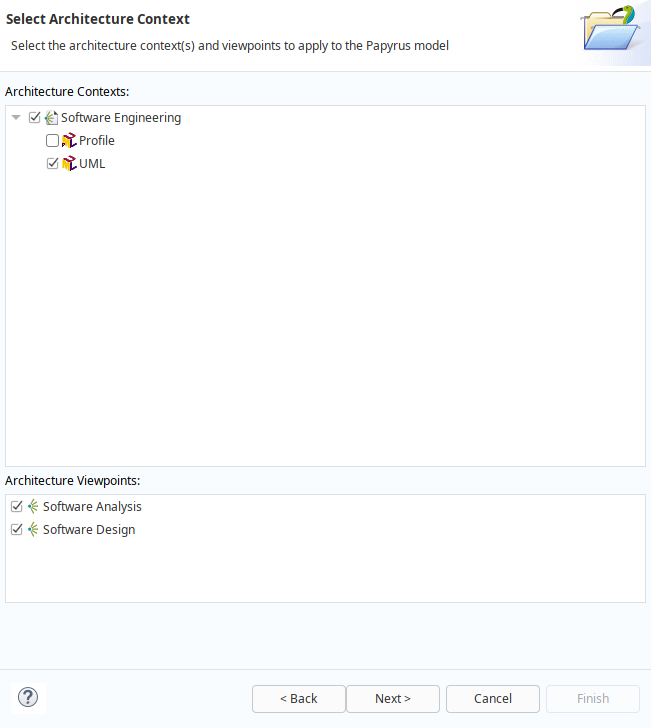
\includegraphics[width=.9\linewidth]{images/project_3.png}
\end{center}
\newpage

In this step, we must choose a name for the project, we will use "Test" in this case:

\begin{center}
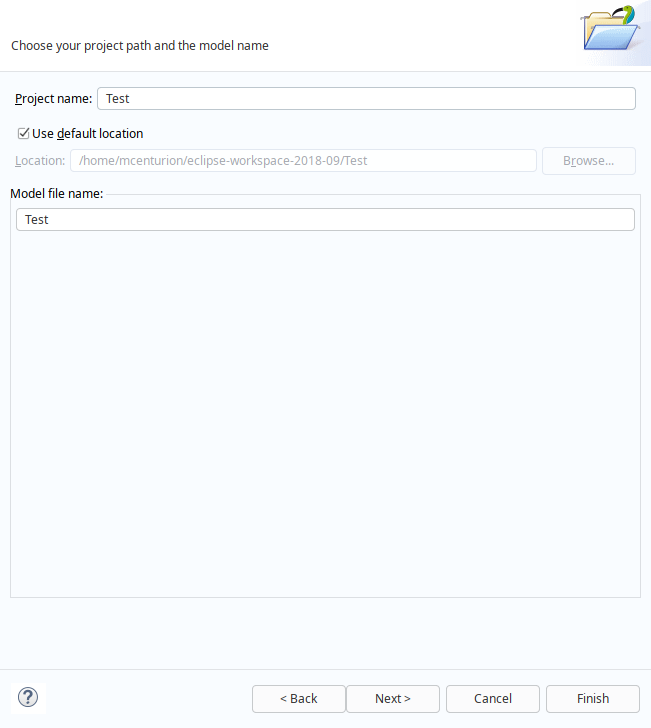
\includegraphics[width=.9\linewidth]{images/project_4.png}
\end{center}
\newpage

In the following window, first we need to select the representation "Deployment Diagram":

\begin{center}
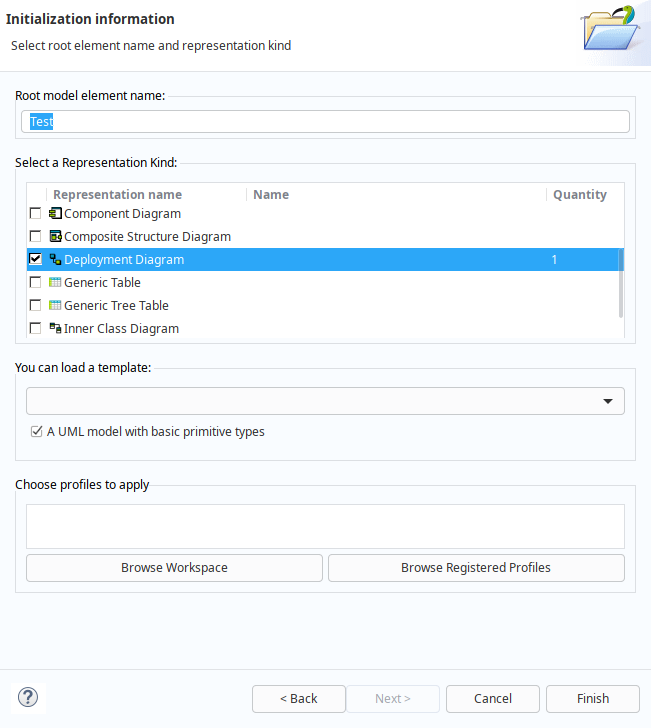
\includegraphics[width=.9\linewidth]{images/project_5.png}
\end{center}
\newpage

Then we need to click "Browse Registered Profiles", and select "MDCMS" in the pop-up window:

\begin{center}
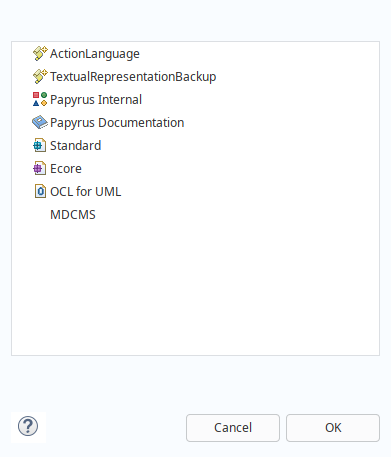
\includegraphics[width=.9\linewidth]{images/project_6.png}
\end{center}

Clicking "Finish" will create our project.
\newpage

\section{Model}
\label{sec:org056320f}

Once the project is created, we will be presented with Papyrus perspective:

\begin{center}
\includegraphics[width=.9\linewidth]{images/modelo_1.png}
\end{center}

From the right panel we will be able to drag and drop elements to the diagram in the center. If we want to represent a PC, we can add a "Device":

\begin{center}
\includegraphics[width=.3\linewidth]{images/modelo_2.png}
\end{center}

By clicking the created element, we will have a "Properties" view available, inside this properties we will also have a "Profile" tab, in which we can click the "+" button in order to add more stereotypes:

\begin{center}
\includegraphics[width=.9\linewidth]{images/modelo_3.png}
\end{center}
\newpage

Since we want to represent a "PC", in the dialog box we need to click "PC" on the left, and the button "->" so we can add said stereotype.


\begin{center}
\includegraphics[width=.9\linewidth]{images/modelo_5.png}
\end{center}

We finally have a PC element in our diagram. All that's left now, is to go to the "Profile" tab, click on the stereotype, and fill in the attributes that are shown:

\begin{center}
\includegraphics[width=.9\linewidth]{images/modelo_6.png}
\end{center}
\newpage

\section{Transformation}
\label{sec:org2b6f134}

Once we have the model created, running the transformation to get the Puppet code is really straightforward.

On the model explorer we need to find the .uml file asociated to our model, and the right click on it:

\begin{center}
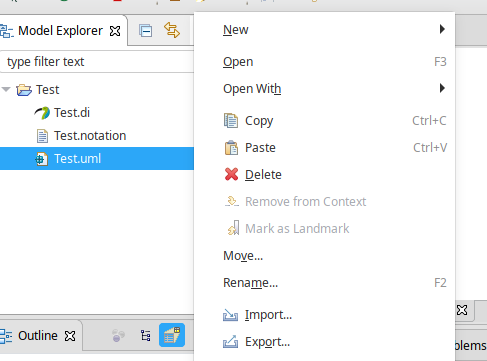
\includegraphics[width=.9\linewidth]{images/transformation_1.png}
\end{center}

At the end of the menu we will have the option "Acceleo Model to Text", where we can select "Generate Mdcm2puppet":

\begin{center}
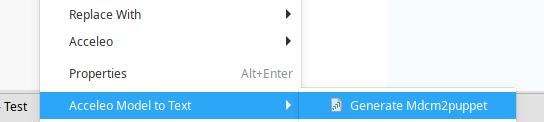
\includegraphics[width=.9\linewidth]{images/transformation_2.png}
\end{center}

By clicking on that option, the transformation will be executed, and once it finishes it will have created a new "src-gen" directory containing the generated code:

\begin{center}
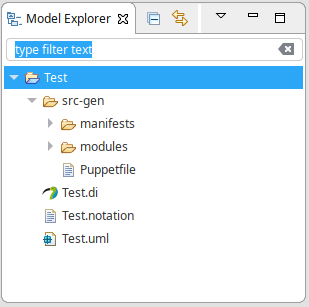
\includegraphics[width=.9\linewidth]{images/transformation_3.png}
\end{center}
\end{document}
